\input{tex/pre} % Ausgelagerte Präambel

% Hier können die Informationen über die Ausarbeitung eingetragen werden
\newcommand*{\Course}{FACH} % Bei vorlesungsbegleitenden Ausarbeitungen
\newcommand*{\Subject}{THEMA}
\newcommand*{\Author}{AUTOR}
\newcommand*{\Matriculation}{MATRIKELNUMMER}
\newcommand*{\Discipline}{STUDIENGANG}
\newcommand*{\Semester}{SEMESTER}
\newcommand*{\Professor}{BETREUER}
\newcommand*{\Deadline}{ABGABETERMIN}
\newcommand*{\Location}{ABGABEORT}

% Um die Übersetzung zu beschleunigen, kann man hiermit nur Teile der Ausarbeitung übersetzen lassen
% \includeonly{FILENAME,FILENAME,...}

% Die folgenden Zeilen können für die Druckausgabe verwendet werden
% Achtung: Durch den vergrößerten Textbereich kann eine erneute Optimierung der Zeilenumbrüche
% notwendig sein.
% \KOMAoptions{BCOR     = 0mm,       % Hier die durchschnittliche Länge eintragen, die durch die
%                                    % Bindung verloren geht
%              DIV      = 11,        % Vergrößerter Textbereich für die Druckausgabe
%              headings = openright, % Kapitel starten immer auf der rechten Seite
%              twoside}
% \ofoot*{\pagemark}
% \ifoot*{}
% \renewcommand*{\Signature}{\rule{6cm}{1pt}\\Unterschrift}

% Metadaten für das PDF
\hypersetup{%
    pdfinfo={%
        Author={\Author\ (Matrikelnummer: \Matriculation)},
        Title={\Subject},
        Subject={\Course},
        Keywords={\Course, \Course, \Author, \Discipline, \Professor}
    }
}

\begin{document}
    \include{tex/titlepage}      % Titelseite
    \cleardoublepage%
\pagestyle{plain}
\pagenumbering{Roman}

\chapter*{Erklärung}
    Ich versichere, dass ich die Ausarbeitung mit dem Thema \enquote{\Subject} selbstständig
    verfasst und keine anderen Quellen und Hilfsmittel als die angegebenen benutzt habe. Die
    Stellen, die anderen Werken dem Wortlaut oder dem Sinn nach entnommen wurden, sind in jedem
    einzelnen Fall unter Angabe der Quelle als Entlehnung (Zitat) kenntlich gemacht. Das Gleiche
    gilt für beigefügte Skizzen und Darstellungen.\\[4cm]
    \parbox{\textwidth}{%
        \parbox[b]{7cm}{%
            \Location, den \today\\[-0.3cm]
            \rule{6cm}{1pt}\\
            Ort, Datum
        }
        \hfill%
        \parbox[b]{7cm}{%
            \Signature%
        }
    }
 % Eidesstattliche Erklärung

    % Hier eigene Kapitel einfügen

	\chapter*{Kurzfassung}
Ziel der Kurzfassung ist es, einen (eiligen) Leser zu informieren, so dass dieser entscheiden kann, ob die Arbeit für ihn hilfreich ist oder nicht (neudeutsch: Management Summary).                               Die Kurzfassung gibt daher eine kurze Darstellung
\begin{itemize}
    \item{des in der Arbeit angegangenen Problems}
    \item{der verwendeten Methode(n)}
    \item{des in der Arbeit erzielten Fortschritts}
\end{itemize}
                                                                     
Dabei sollte nicht auf die Struktur der Arbeit eingegangen werden, also Kapitel 2 etc. denn die Kurzfassung soll ja gerade das Wichtigste der Arbeit vermitteln, ohne dass diese gelesen werden muss. Eine Kapitelbezogene Darstellung sollte sich in Kapitel 1 unter Vorgehen befinden.

Länge: Maximal 1 Seite.

    \include{tex/frontmatter}    % Verzeichnisse, Vorbereitung Layout eigene Kapitel


	\chapter*{Abbildungsverzeichnis}
Abbildung 1: Vorgehen nach (1)
		\newpage
	
	\chapter*{Abbildungsverzeichnis}
Tabelle 1: Testtabelle
		\newpage

	\chapter*{Abkürzungssverzeichnis}
		\newpage

	\chapter{Einleitung}
Die Einleitung dient dazu, beim Leser Interesse für das Thema der Arbeit zu wecken, das behandelte Problem aufzuzeigen und den zu seiner Lösung eingeschlagenen Weg zu beschreiben.
		\section{Motivation}
In der Motivation wird dargestellt, wieso es notwendig ist, sich mit dem in der Arbeit identifizierten und behandelten Problem zu beschäftigen.
		\section{Problemstellung und -abgrenzung}
Die Problemstellung beginnt mit der Einordnung in ein thematisches Umfeld und enthält sowohl die in der Arbeit angegangenen Problempunkte, als auch weitere, nicht behandelte Problempunkte. Eine Negativabgrenzung verhindert, dass beim Leser später nicht erfüllte Erwartungen geweckt werden.
		\section{Ziel der Arbeit}
Mit dem Ziel der Arbeit wird der angestrebte Lösungsansatz festgelegt. An diesem Ziel wird die Arbeit gemessen.Mit dem Ziel der Arbeit wird der angestrebte Lösungsansatz festgelegt. An diesem Ziel wird die Arbeit gemessen.
		\section{Vorgehen}
Nachdem mit Problemstellung und Ziel gewissermaßen Anfangs- und Endpunkt der Arbeit beschrieben sind, wird hier der zur Erreichung des Ziels eingeschlagene Weg vorgestellt. Dazu werden typischerweise die folgenden Kapitel und ihr Beitrag zur Erreichung des Ziels der Arbeit kurz beschrieben. Die folgenden Kapitel sind ein – möglicher – Aufbau, Abweichungen können durchaus notwendig sein. Zur Darstellung des Vorgehens kann eine grafische Darstellung sinnvoll sein, bei der die einzelnen Lösungsschritte und ihr Zusammenhang dargestellt werden. Ein Beispiel hierfür findet sich in \hyperlink{Abbildung1}{Abbildung1}.

	\newpage
	\begin{figure}[h]
	\centering
	\hypertarget{Abbildung1}{}
	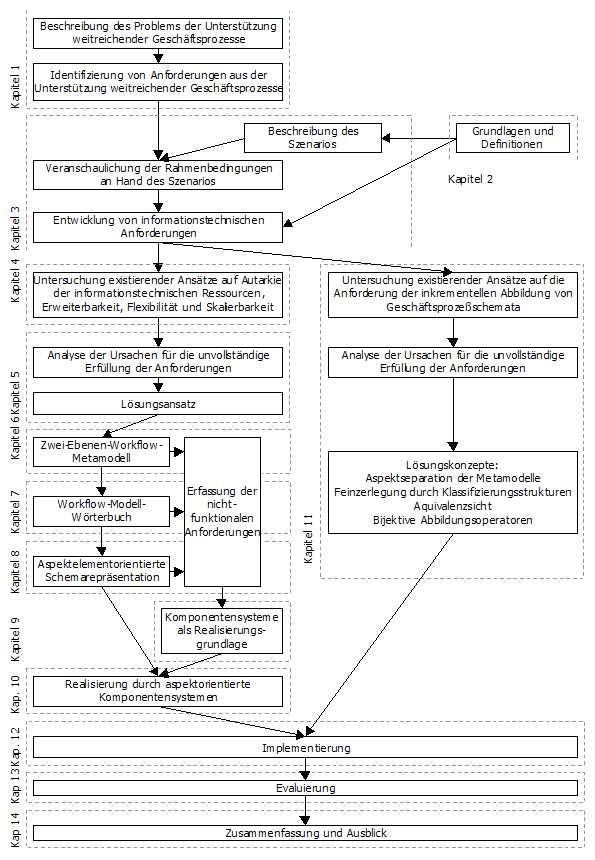
\includegraphics{img/Abbildung1.png}
	\caption{Vorgehen nach \protect \hyperlink{[1]}{[1]}}
	\end{figure}
	\newpage

	\chapter{Grundlagen}
In diesem Kapitel werden für die weitere Arbeit wichtige Begriffe eingeführt. Dabei ist darauf zu achten, nur solche Inhalte in das Grundlagenkapitel aufzunehmen, die später auch verwendet werden (Problembezogenheit). Ebenso ist auf eine ausreichend tiefe und vollständige Darstellung der Grundlagen zu achten.
	\newline \newline
Für die Erstellung des Literaturverzeichnisses wird das Werkzeug Zotero \href{www.zotero.org}{www.zotero.org} verwendet. Das Literaturverzeichnis in dieser Vorlage wurde mit Zotero gemäß dem IEEE Format erstellt. 
	\newline \newline
Hilfreich kann der Vergleich von Definitionen mit Hilfe einer Tabelle sein, wie in \hyperlink{tabelle1}{Tabelle 1} dargestellt.
	\newline
	\begin{figure}[h]
	\hypertarget{tabelle1}{}
	\begin{tabularx}{\columnwidth}{|X|X|}
	\hline
	Definition 1 & ... \\
	\hline
	Definition 2 & ... \\
	\hline
	\end{tabularx}
	\caption{Testtabelle}
	\end{figure}
		\section{Grundlagengebiet A}
			\subsection{Definition AA}
			\subsection{Definition AB}
		\section{Grundlagengebiet B}
			\subsection{Definition BA}
			\subsection{Definition BB}
		\newpage

	\chapter{Hauptteil (1. Kapitel)}
Für die Gestaltung des Hauptteils sind in Abhängigkeit von der Aufgabenstellung unterschiedliche Ausformungen möglich. In den Richtlinien zu Studien- und Diplomarbeiten finden Sich hierzu Erläuterungen.
		\newpage

	\chapter{Hauptteil (2. Kapitel)}
		\newpage

	\chapter{Hauptteil (3. Kapitel)}
		\newpage

	\chapter{Evaluierung}
Aufgabe des Kapitels Evaluierung ist es, aufzuzeigen in wie weit die Ziele der Arbeit erreicht wurden. Es sollen also die erreichten Arbeitsergebnisse mit den Zielen verglichen werden. Ergebnis der Evaluierung kann auch sein, das bestimmte Ziele nicht erreicht werden konnten, wobei die Ursachen hierfür auch außerhalb des Verantwortungsbereichs des Autors liegen können.
		\newpage

	\chapter{Zusammenfassung und Ausblick}
		\section{Erreichte Ergebnisse}
Die Zusammenfassung dient dazu, die wesentlichen Ergebnisse der Arbeit und vor allem die entwickelte Problemlösung und den erreichten Fortschritt darzustellen. (Sie haben Ihr Ziel er-reicht und dies nachgewiesen).
		\section{Ausblick}
Im Ausblick werden Ideen für die Weiterentwicklung der erstellten Lösung aufgezeigt. Der Aus-blick sollte daher zeigen, dass die Ergebnisse der Arbeit nicht nur für die in der Arbeit identifi-zierten Problemstellungen verwendbar sind, sondern darüber hinaus erweitert sowie auf andere Probleme übertragen werden können.
    			\subsection{Erweiterbarkeit der Ergebnisse}
    			\subsection{Übertragbarkeit der Ergebnisse}
		\newpage

	\chapter{Literaturverzeichnis}
\hypertarget{[1]}{[1]} \href{http://digbib.ubka.uni-karlsruhe.de/volltexte/91999}{R. Schmidt, “Aspektorientierte Komponentensysteme zur Unterstützung weitreichender Geschäftsprozesse,” 2000, S. 10; http://digbib.ubka.uni-karlsruhe.de/volltexte/91999.}
		\section*{Anlage 1}
		\addcontentsline{toc}{section}{Anlage 1}
		\section*{Anlage 2}
		\addcontentsline{toc}{section}{Anlage 2}
		

\end{document}
